\chapter{Effetto Hall quantistico}
L'effetto Hall classico fu scoperto nel 1879 da E. Hall studiando le proprietà dei conduttori in presenza di campi magnetici. Si consideri un conduttore lungo e sottile percorso da una corrente $I$ immerso in un campo magnetico $\vB$ perpendicolare al conduttore. A causa del campo $\vB$, gli elettroni percepiscono l'azione del campo magnetico tramite una forza di Lorentz che tende a farli deviare verso uno dei due bordi del conduttore. L'effetto di questo spostamento di cariche è la comparsa di una differenza di potenziale trasversale $V_H$, la quale è legata alla resistenza di Hall $R_H$ tramite la legge di Ohm
\begin{equation}
    R_H = \frac{V_H}{I},
\end{equation}
che a sua volta risulta essere proporzionale al campo magnetico che l'ha prodotta. Questo fenomeno ha avuto diverse applicazione pratiche ed in particolare è stato sfruttato per costruire sonde in grado di misurare campi magnetici attraverso semplici misure di tensione. Poco dopo la scoperta di Hall, von Klitzing notò che il comportamento di $R_H$ a temperature nell'ordine del Kelvin mostrava un comportamento radicalmente diverso da quello previsto classicamente. In queste condizioni, $R_H$ non varia più con continuità rispetto al campo magnetico applicato, ma assume soltanto un insieme discreto di valori, dati da
\begin{equation}
\label{eq: resistenza di Hall quantizzata}
    R_H = \frac{h}{\nu e^2} \equiv \frac{R_K}{\nu},\quad \nu \in \N,
\end{equation}
dove $R_K$ è la costante di von Klitzing. La spiegazione teorica di questo andamento, verificato sperimentalmente con precisioni dell'ordine di $10^{-9}$, è stata fornita da Laughlin poco dopo l'osservazione di von Klitzing. L'interpretazione dei dati sperimentali si basava sulle proprietà quantistiche universali dei singoli elettroni quando sono confinati a muoversi in due dimensioni e sono immersi in un campo magnetico perpendicolare alla direzione del loro moto. In queste condizioni, come già previsto da Landau, gli elettroni possiedono uno spettro discreto descritto da un opportuno oscillatore armonico, dove il numero di livelli completamente occupati è proprio il numero quantico $\nu$ presente nella relazione trovata da von Klitzing in equazione \eqref{eq: resistenza di Hall quantizzata}. In quegli stessi anni, Tsui, Stomer e Gossard scoprirono l'effetto Hall frazionario dove il numero intero $\nu$ viene sostituito da un numero frazionario $u$ nella relazione \eqref{eq: resistenza di Hall quantizzata}, ossia
\begin{equation}
    R_H = \frac{R_K}{u},\quad u \in \mathbb{Q}.
\end{equation}

La resistenza e la resistività sono legate dalla seconda legge di Ohm 
\begin{equation}
    R = \frac{\rho L}{A},
\end{equation}
dove $L$ è la lunghezza del conduttore e $A$ la sua sezione. In generale, considerando un ipercubo di lato $L$, ossia un cubo $D$-dimensionale, la resistenza è 
\begin{equation}
    R = \frac{\rho L}{L^{D - 1}} = \rho L^{2 - D}.
\end{equation}
Da questo si vede che il caso bidimensionale è peculiare dato che resistenza e resistività coincidono, in particolare $R$ è un invariante di scala e $e^2R/h$ è una quantità adimensionale. Questa proprietà è centrale per l'universalità dei risultati dato che non c'è bisogno di misurare le dimensioni del campione in modo estremamente preciso per ottenere la resistività alla precisione richiesta nel caso tridimensionale.

\section{Carica in un campo magnetico}
L'equazione del moto di un elettrone di carica $-e$, di massa $m$ e velocità $\vv$ soggetto alla forza di Lorentz dovuta ad un campo magnetico $\vB$ è
\begin{equation}
    m\frac{d\vv}{dt} = - e(\vv \times \vB).
\end{equation}
Se il campo magnetico è $\vB = B\,\hat{u}_z$ e la velocità iniziale è nel piano $(x,y)$, allora il moto è confinato in tale piano e il problema è bidimensionale. Date le coordinate $x_i \equiv (x_1,x_2) = (x,y)$ e le componenti della velocità $v_i \equiv (v_1,v_2) = (v_x,v_y)$ della particella si può scrivere l'equazione del moto come
\begin{equation}
    m\frac{dv_i}{dt} = -eB\epsilon_{ij}v_j = -m\omega_c\epsilon_{ij}v_j,
\end{equation}
dove $\omega_c = eB/m$ è la frequenza di ciclotrone, o di Larmor. Questa equazione si può riscrivere a sua volta come una derivata totale
\begin{equation}
    \frac{d}{dt}(p_i + m\omega_c\epsilon_{ij}x_j) = 0,
\end{equation}
da cui si deduce che il sistema possiede due costanti del moto 
\begin{equation}
    Q_i = p_i + m\omega_c\epsilon_{ij}x_j.
\end{equation}
Introducendo quindi la combinazione complessa $p = p_1 + ip_2$ si ha 
\begin{equation}
    \begin{cases}
        \dfrac{dp_1}{dt} = -\omega_cp_2 \\[2ex]
        i\dfrac{dp_2}{dt} = i\omega_cp_1
    \end{cases},
\end{equation}
che porta all'equazione differenziale 
\begin{equation}
\label{eq: equazione del moto di un carica in un campo B}
    \frac{dp}{dt} = i\omega_cp,
\end{equation}
la cui soluzione è
\begin{equation}
    p(t) = p_0e^{i\omega_c t},
\end{equation}
pertanto, dividendo per $m$ e integrando la velocità, si trova che la traiettoria della particella è 
\begin{equation}
    x(t) = x_1(t) + ix_2(t) = \frac{v_0}{i\omega_c}e^{i\omega_c t} + x_0 -   \frac{v_0}{i\omega_c}.
\end{equation}
Dunque, il moto è circolare uniforme con velocità angolare $\omega_c$ e raggio $R = v_0m/eB$.

Se ora al sistema si aggiunge un campo elettrico $\vE$ parallelo al piano $(x,y)$, l'equazione del moto diventa
\begin{equation}
    m\frac{d\vv}{dt} = -e(\vv \times \vB + \vE),
\end{equation}
o in forma complessa 
\begin{equation}
    \frac{dp}{dt} = i\omega_c\bigg(p - \frac{eE}{i\omega_c}\bigg),\quad E= E_1 + iE_2,
\end{equation}
la quale ponendo $\xi = p - eE/i\omega_c$, assume la medesima forma dell'equazione \eqref{eq: equazione del moto di un carica in un campo B} trovata prima; infatti si ha
\begin{equation}
    \frac{d\xi}{dt} = i\omega_c\xi,
\end{equation}
da cui si ricava immediatamente
\begin{equation}
\label{eq: velocità carica in campo EM}
    v(t) = v_0e^{i\omega_c t} + \frac{eE}{im\omega_c} = v_0e^{i\omega_c t} + \frac{E}{iB}.
\end{equation}
Il secondo termine in equazione \eqref{eq: velocità carica in campo EM} è chiamato ``velocità di trascinamento'' degli elettroni e indicato con $v_T$, la quale è dovuta alla presenza del campo elettrico $\vE$. Associata alla velocità di trascinamento è la densità di corrente
\begin{equation}
    \vJ = -en_e\vv_T = -\frac{en_e\vE}{iB},
\end{equation}
dove $n_e$ è la densità di elettroni, le cui componenti sono 
\begin{equation}
    J_x = -\frac{en_eE_y}{B},\quad J_y = \frac{en_eE_x}{B}.
\end{equation}
Quindi, la densità di corrente è perpendicolare al campo elettrico. Inoltre in generale, in un conduttore qualsiasi esiste una relazione lineare tra la densità di corrente e il campo elettrico della forma
\begin{equation}
    \begin{pmatrix}
        J_x \\
        J_y
    \end{pmatrix} = 
    \begin{pmatrix}
        \sigma_{xx} & \sigma_{xy} \\
        \sigma_{yx} & \sigma_{yy}
    \end{pmatrix}
    \begin{pmatrix}
        E_x \\
        E_y
    \end{pmatrix},
\end{equation}
oppure nella forma
\begin{equation}
    \begin{pmatrix}
        E_x \\
        E_y
    \end{pmatrix} = 
    \begin{pmatrix}
        \rho_{xx} & \rho_{xy} \\
        \rho_{yx} & \rho_{yy}
    \end{pmatrix}
    \begin{pmatrix}
        J_x \\
        J_y
    \end{pmatrix}.
\end{equation}
In particolare, per l'effetto Hall nel vuoto o in un conduttore ideale si ha che 
\begin{equation}
    \sigma_{xx} = \sigma_{yy} = 0,\quad \rho_{xx} = \rho_{yy} = 0, 
\end{equation}
mentre la conduttività di Hall è
\begin{equation}
    \sigma_H \equiv \sigma_{yx} = -\sigma_{xy} = \frac{n_ee}{B},
\end{equation}
tramite la quale si può scrivere la componente $x$ della densità di corrente $J$ come 
\begin{equation}
    J_x = -\sigma_H E_y.
\end{equation}
In un conduttore a forma di nastro di larghezza $L$, indicando con $V_y = -E_yL$ la differenza di potenziale tra i bordi e con $I_x = J_xL$ la corrente che scorre lungo l'asse $x$, si può scrivere
\begin{equation}
    \sigma_H = \frac{I_x}{V_y} = -\frac{\sigma_x}{E_y} = \frac{n_ee}{B},
\end{equation}
da cui 
\begin{equation}
\label{eq: resistenza di Hall classica}
    R_H = \frac{B}{n_ee}.
\end{equation}
Questo risultato si lega all'affermazione iniziale secondo cui la resistenza di Hall $R_H$ di un sistema classico tridimensionale cresce linearmente con l'intensità del campo magnetico che l'ha generata, a differenza di quanto accade in un sistema bidimensionale, come mostrato in figura \ref{fig: EH 3D vs 2D}.
\begin{figure}[h]
    \centering
    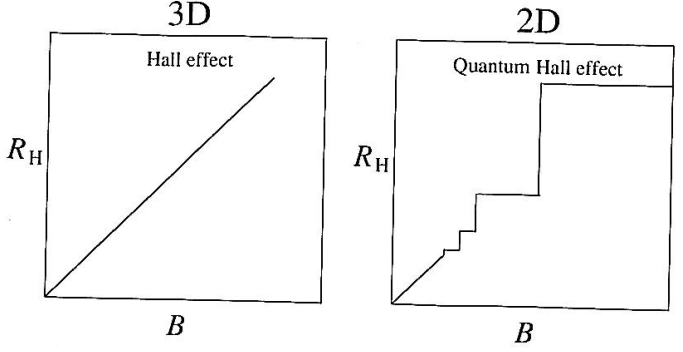
\includegraphics[width=0.6\linewidth]{Immagini - Capitolo 3/EH 3D vs 2D.png}
    \caption{differenza tra l'effetto Hall in tre dimensioni e in due dimensioni.}
    \label{fig: EH 3D vs 2D}
\end{figure}

\section{Livelli di Landau}
L'hamiltoniana per un elettrone non relativistico che si muove su un piano attraversato da un campo magnetico perpendicolare è
\begin{equation}
    \hatH = \frac{1}{2m}(\hatp + e\vA)^2.
\end{equation}
Se il campo magnetico è costante, allora vale che $\nabla \times \vA = B\,\hatz$, ossia che $\vA$ è lineare nelle coordinate $x$ ed $y$. Questo implica che l'hamiltoniana precedente è quella che descrive un oscillatore armonico e può pertanto essere diagonalizzata in modo esatto. Dato che l'equazione di Schr\"odinger è invariante per trasformazioni di gauge locali a causa della presenza del campo magnetico, è conveniente fissare il gauge, le scelte più usate sono:
\begin{enumerate}
    \item il gauge di Landau dove $\vA = B(-y,0,0)$ per geometrie a nastro;
    \item il gauge simmetrico dove $\vA = (B/2)(-y,x,0)$ per geometrie a disco.
\end{enumerate}

\subsection{Gauge di Landau}
In questo caso l'hamiltoniana non contiene termini dipendenti dalla coordinata $x$ e pertanto commuta con $p_x$. Questa proprietà implica che la funzione d'onda totale può essere fattorizzata come
\begin{equation}
    \eta(x,y) = \mathcal{N}e^{ik_xx}\phi(y).
\end{equation}
L'hamiltoniana del sistema può quindi essere scritta come
\begin{equation}
    \hatH = \frac{1}{2m}[p_y^2 + (\hbar k_x - eBy)^2].
\end{equation}
Conviene adesso introdurre le quantità
\begin{equation}
    l \equiv \sqrt{\frac{\hbar}{eB}},\quad y' \equiv \frac{y}{l} -lk_x,\quad p_y' \equiv \frac{lp_y}{\hbar},
\end{equation}
così da poter riscrivere l'hamiltoniana come
\begin{equation}
    \hatH = \hbar\omega_c\bigg(\frac{p_y'^2}{2}+ \frac{y'^2}{2}\bigg).
\end{equation}
Quindi, i livelli di energia quantizzati, detti livelli di Landau, sono 
\begin{equation}
    E_n = \hbar\omega_c\bigg(n + \frac{1}{2}\bigg),\quad n \in \N.
\end{equation}
In pratica, il continuo di livelli di energia presenti a $B = 0$, in presenza di un campo magnetico si combinano in modo tale da formare livelli di Landau degeneri, come mostrato in figura \ref{fig: livelli di Landau}. Se l'energia è quantizzata, un elettrone in un dato livello non può variare in modo continuo la sua energia cinetica, quindi la conservazione dell'energia lo vincola su linee equipotenziali. Si noti che l'energia non dipende da $k_x$, per cui autostati che differiscono solo in tale quantità e non in $n$ sono degeneri, mentre la posizione del centro dell'oscillatore dipende da $k_x$; infatti le autofunzioni sono
\begin{equation}
    \eta_{n,k_x} = \mathcal{N}e^{ik_xx}\exp{\bigg[-\frac{1}{2}\bigg(\frac{y}{l} - lk_x\bigg)^2\bigg]}H_x\bigg(\frac{y}{l} - lk_x\bigg),
\end{equation}
dove $H_n$ sono i polinomi di Hermite, localizzate attorno a $y_0(k_x) = l^2k_x \equiv y_0$.  
\begin{figure}[H]
    \centering
    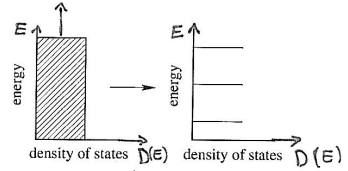
\includegraphics[width=0.5\linewidth]{Immagini - Capitolo 3/livelli di Landau.png}
    \caption{il mare di Fermi diviso in livelli di Landau equispaziati e degeneri in seguito all'applicazione del campo magnetico.}
    \label{fig: livelli di Landau}
\end{figure}

Quindi, lungo la direzione dell'asse $x$ si ha un'onda piana, mentre lungo la direzione dell'asse $y$ l'elettrone è localizzato e la traiettoria seguita è una linea retta centrata in $y_0(k_x)$. Cambiare valore di $k_x$ significa quindi cambiare traiettoria spostandosi verso il basso o verso l'alto, visualizzando così i momenti nello spazio delle coordinate. In particolare se si considera una geometria dove la direzione $x$ è periodica con lunghezza $L_x$, come ad esempio un cilindro la cui base ha lunghezza $L_x$, allora 
\begin{equation}
    k_x = \frac{2\pi}{L_x}n_x,\quad n_x \in \Z
\end{equation}
e la distanza tra i centri delle gaussiane, ossia la differenza tra le traiettorie seguite dagli elettroni, è 
\begin{equation}
    \Delta y_0 = \frac{2\pi l^2}{L_x}.
\end{equation}
Ricapitolando, introducendo un campo magnetico ortogonale alla geometria si è passati da un continuo di livelli energetici ad un insieme discreto di essi dato dai livelli di Landau, dove per $n = 0$ si ha il livello fondamentale associato all'oscillatore armonico. Quest'ultimo diventa infinitamente popolato se il volume della geometria è infinito, ma se questo non è il caso allora, dato che i momenti corrispondono a posizioni, si può dedurre che ogni livello di Landau non sia infinitamente popolato, ma sarà degenere e quindi dotato di un numero massimo di stati accessibili. Nel gauge di Landau gli orbitali degeneri sono etichettati dai numeri quantici $k_x$ e $n \in \N$. La degenerazione per unità di area è la stessa in ogni livello di Landau, ma dipende dal campo magnetico $\vB$. Per trovare la degenerazione si considera nuovamente la geometria data dal cilindro di dimensioni $L_x$ ed $L_y$, la cui periodicità permette di scrivere
\begin{equation}
    e^{ik_x(x + L_x)} = e^{ik_xx},
\end{equation}
per cui gli stati permessi sono dati da
\begin{equation}
    k_x = \frac{2\pi n_x}{L_x},\quad n_x \in \Z.
\end{equation}
Poiché il centro delle gaussiane è dato da $y_0$, solo gli stati con $0 < y_0 < L_y$ sono permessi, quindi per $y_0 = L_y$ si ha
\begin{equation}
    \frac{L_y}{l^2} = k_x^{(max)} = \frac{2\pi}{L_x}n_x^{(max)},
\end{equation}
ossia 
\begin{equation}
    n_x^{(max)} = \frac{L_yL_x}{2\pi l^2},
\end{equation}
che corrisponde quindi al numero massimo di stati nell'area $L_xL_y$. Pertanto, la degenerazione per unità di area è 
\begin{equation}
    \frac{n_x^{(max)}}{L_xL_y} = \frac{1}{2\pi l^2} = \frac{eB}{2\pi\hbar} = \frac{B}{\Phi_0}, 
\end{equation}
per cui
\begin{equation}
    n_x^{(max)} = \frac{\Phi}{\Phi_0}
\end{equation}
e in un livello di Landau ci può stare al più un elettrone per quanto di flusso di campo magnetico. Si può definire poi il fattore di riempimento come
\begin{equation}
    \nu = \frac{n_e\Phi_0}{B} = \frac{n_e\Phi_0L_xL_y}{BL_xL_y} \equiv \frac{\mathrm{\#\,di\,elettroni}}{\mathrm{\#\,di\,flussoni}}.
\end{equation}
Sostituendo $B = n_e\Phi_0/\nu = n_eh/e\nu$ nell'espressione di $R_H$ in \eqref{eq: resistenza di Hall classica} si trova la relazione di von Klitzing
\begin{equation}
    R_H = \frac{h}{\nu e^2}.
\end{equation}
I valori di $R_H$ osservati sperimentalmente in corrispondenza dei plateau sono 
\begin{equation}
    R_H = \frac{h}{ne^2},\quad n \in \N,
\end{equation}
come se il sistema, in corrispondenza dei plateau, avesse un fattore di riempimento $\nu$ intero anche se il campo magnetico sta variando. Le transizioni tra un plateau e l'altro avvengono in corrispondenza dei valori interi di $\nu$, mentre $\rho_{xx} \simeq 0$ diminuendo di un fattore $10^{-13}$ e presentando picchi in corrispondenza delle transizioni tra plateau.
\begin{figure}[h]
    \centering
    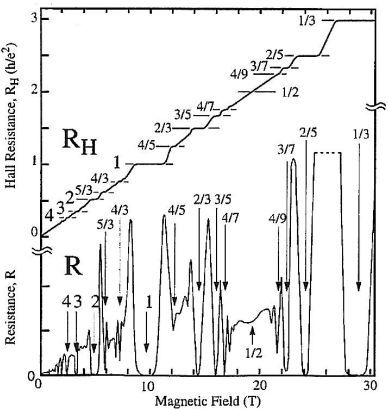
\includegraphics[width=0.49\linewidth]{Immagini - Capitolo 3/resistenze di Hall.png}
    \caption{valori sperimentali di $R_H$.}
    \label{fig: resistenze di Hall}
\end{figure}

\subsubsection{Splitting dei livelli energetici}
Quando il nastro è percorso da una corrente $I_x$ si manifesta una differenza di potenziale $\Delta V = -E_yL_y$ tra i due bordi e l'hamiltoniana del singolo elettrone nel gauge di Landau diventa
\begin{equation}
    \hatH =-\frac{\hbar^2}{2m}\frac{d^2}{dy^2} + \frac{m\omega^2_c}{2}(y - y_0)^2 + eyE_y,\quad y_0 = l^2k_x = \frac{\hbar k_x}{eB}.
\end{equation}
Questa continua ad essere l'hamiltoniana di un oscillatore armonico e ridefinendo il centro del sito di Landau come
\begin{equation}
    y_0 \to \tilde{y}_0 = y_0 - \frac{eE_y}{\omega_c^2 m}
\end{equation}
si ottiene
\begin{equation}
    \hatH = -\frac{\hbar^2}{2m}\frac{d^2}{dy^2} + \frac{m\omega_c^2}{2}(y_0 - \tilde{y}_0)^2 + eE_y\tilde{y}_0(k_x) + \frac{mE_y^2}{2B^2}.
\end{equation}
Lo spettro dei possibili livelli energetici risulta pertanto essere
\begin{equation}
\label{eq: legge dispersione livelli di Landau con campo E}
    E_{n,k_x} = \hbar\omega_c\bigg(n + \frac{1}{2}\bigg) + eE_y\tilde{y}_0(k_x) + \frac{mE_y^2}{2B^2}.
\end{equation}
Tale spettro ora dipende da entrambi i numeri quantici $n$ e $k_x$, mentre la presenza del campo elettrico $E_y$ rimuove completamente la degenerazione dei livelli energetici, infatti l'energia dipende esplicitamente dalla coordinata $\tilde{y}_0(k_x)$ del sito di Landau. Inoltre, per $B \gg E_y$, lo splitting dovuto al campo elettrico è trascurabile rispetto a $\hbar\omega_c = \hbar eB/m$ e quindi si trascura la possibilità di avere livelli di energia degeneri con numero quantico $n$ diverso. Tuttavia, nella geometria finita considerata bisogna tenere conto anche delle deformazione dei livelli ai bordi del sistema, come mostrato in figura \ref{fig: livelli energetici}.
\begin{figure}[h]
    \centering
    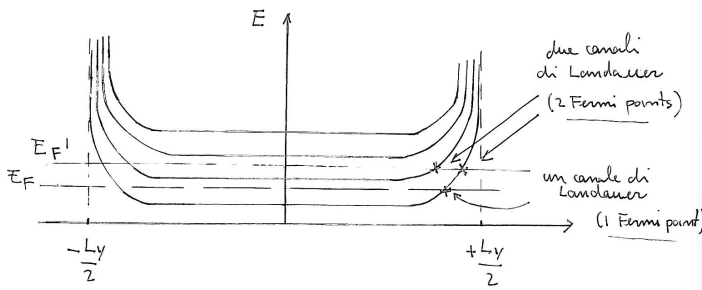
\includegraphics[width=0.7\linewidth]{Immagini - Capitolo 3/livelli energetici.png}
    \caption{livelli energetici per una geometria finita.}
    \label{fig: livelli energetici}
\end{figure}

Immaginando di avere il primo livello di Landau completamente riempito, gli unici elettroni che possono muoversi quando ricevono energia sono quelli ai bordi del conduttore. Questi elettroni possono muoversi praticamente lungo un'unica dimensione, dando luogo ad un tipo di conduzione detta ``balistica''. Per questo motivo la resistività $\rho_{xx}$ sui plateau è quasi nulla e le correnti possono resistere per solo per tempi sulla scala dei minuti, invece che per un tempo indefinito come accade per i superconduttori. Inoltre, la conduzione balistica differisce dalla superconduttività per l'assenza dell'effetto Meissner-Ochsenfeld.

Tuttavia, quanto detto non spiega la formazione dei plateau. Per spiegare la loro presenza si devono considerare le impurità nel reticolo, le quali contribuiscono allo splitting dei livelli di Landau anche in assenza del campo elettrico $E_y$, generando degli stati localizzati tra i livelli di Landau. Ad esempio, si supponga di avere il primo livello di Landau completamente riempito, gli elettroni anche avendo la possibilità di saltare al livello di Landau superiore, sono confinati dalle impurità al primo livello. Aumentando il fattore di riempimento, ad esempio diminuendo il campo magnetico $B$, gli elettroni migrano su stati localizzati e non partecipano alla corrente.

\subsubsection{Formula di von Klitzing}
A questo punto è possibile derivare la formula di von Klitzing per la corrente di Hall in presenza di impurità
\begin{equation}
\label{eq: formula di von Klitzing}
    I_H = \frac{e^2\nu}{h}V_H.
\end{equation}
Concentrandosi sul caso in cui $\nu = 1$, per $E_y = 0$, il campo magnetico agisce sugli elettroni facendogli seguire delle orbite circolari chiuse con frequenza $\omega_c$, per cui il trasporto di corrente avviene unicamente sui bordi del conduttore, come mostrato pittoricamente in figura \ref{fig: formula von Klitzing}. Inoltre, se $V_H = 0$, le due correnti sui bordi sono identiche in modulo e di verso opposto, confluendo quindi in una corrente netta nulla. 
\begin{figure}[h]
    \centering
    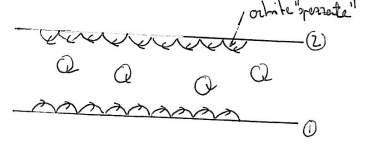
\includegraphics[width=0.5\linewidth]{Immagini - Capitolo 3/formula von Klitzing.png}
    \caption{trasporto di corrente in assenza di campo elettrico $E_y$.}
    \label{fig: formula von Klitzing}
\end{figure}

Invece, se $E_y = \mathrm{costante}$, allora la legge di dispersione per il primo livello di Landau, trovata in equazione \eqref{eq: legge dispersione livelli di Landau con campo E}, è
\begin{equation}
    \epsilon(k_x) = E_{0,k_x} = \frac{\hbar\omega_c}{2} + e\tilde{y}_0(k_x)E_y + \frac{mE_y^2}{2B^2}.
\end{equation}
Quindi, la velocità di gruppo nella direzione $x$ è
\begin{equation}
    v_{k_x} = \frac{1}{\hbar}\frac{\p\epsilon(k_x)}{\p k_x} = \frac{eE_y}{\hbar}\frac{\p\tilde{y}_0(k_x)}{\p k_x} = \frac{eE_yl^2}{\hbar} = \frac{E_y}{B},
\end{equation}
che coincide proprio con la velocità di trascinamento $v_T \equiv E_y/B$ ed pertanto indipendente da $k_x$.

Considerando adesso il caso in cui, a causa della presenza di impurità, il campo elettrico è una funzione $E_y \equiv E_y(y)$, la legge di dispersione restituisce
\begin{equation}
    \epsilon(k_x) = \frac{\hbar\omega_c}{2} + e\tilde{y}_0E_y(\tilde{y}_0) + \frac{mE_y(\tilde{y}_0)^2}{2B^2},\quad \tilde{y}_0 \equiv \tilde{y}_0(k_x),
\end{equation}
mentre la velocità di gruppo è nuovamente data da
\begin{equation}
    v_{k_x} = \frac{1}{\hbar}\frac{\p\epsilon(k_x)}{\p k_x},
\end{equation}
con la quale si può calcolare la corrente che percorre il dispositivo
\begin{equation}
    I_H = -e\int\frac{dk_x}{2\pi}\frac{1}{\hbar}\frac{\p\epsilon(k_x)}{\p k_x}\eta_{k_x}.
\end{equation}
Se lo stato è completamente occupato, allora $\eta_{k_x}$, che corrisponde alla probabilità che lo stato $k_x$ sia occupato, è pari ad uno, per cui la corrente risulta essere
\begin{equation}
    I_H = -\frac{e}{h}[\mu(L_y) - \mu(0)] = \frac{e^2}{h}V_H.
\end{equation}
Quindi, nel caso di $\nu$ generico, $\eta_{k_x}$ viene sostituito da $\nu \eta_{k_x}$ e la corrente assume la forma
\begin{equation}
    I_H = \frac{e^2\nu}{h}V_H,
\end{equation}
che è proprio la formula di von Klitzing per la corrente di Hall in equazione \eqref{eq: formula di von Klitzing}.

\subsubsection{Gedanken experiment di Laughlin}
Si consideri un dispositivo di Hall a forma di disco bucato al centro. Si supponga di instaurare un flusso di campo magnetico $\Phi(t)$ attraverso il foro del dispositivo, il quale viene incrementato adiabaticamente nel tempo da 0 a $\Phi_0$. Per la legge di Faraday, un cambiamento del flusso di campo magnetico induce un campo elettrico dato da
\begin{equation}
    \oint_\Gamma d\vl \cdot \vE = -\frac{\p\Phi(t)}{\p t},
\end{equation}
dove l'integrale viene considerato su un cammino chiuso che circonda il foro del disco. Dato che non si ha dissipazione e che $\sigma_{xx} = \sigma_{yy} = \rho_{xx} = \rho_{yy} = 0$, il campo elettrico induce una densità di corrente
\begin{equation}
    \vE = \rho_{xy}(\vJ \times \hatz) = (\rho_{xy}J_y,0,0),
\end{equation}
quindi la legge di Faraday si riscrive come
\begin{equation}
    \rho_{xy}\oint_\Gamma (\hatz \cdot d\vl) \cdot \vJ = -\frac{d\Phi(t)}{dt},
\end{equation}
dove l'integrale nel membro di sinistra rappresenta la corrente totale che fluisce all'interno della regione delimitata dal percorso $\Gamma$, potendo quindi scrivere
\begin{equation}
    \rho_{xy}\frac{dQ(t)}{dt} = -\frac{d\Phi(t)}{dt},
\end{equation}
la quale integrata tra $t = 0$ dove $\Phi = 0$ e $t'$ dove $\Phi = \Phi_0$ restituisce
\begin{equation}
    \rho_{xy}Q = -\Phi_0.
\end{equation}
Quindi, la carica può essere scritta in funzione del fattore di riempimento
\begin{equation}
    Q = \sigma_{xy}\Phi_0 = \frac{h}{e}\sigma_{xy} = \nu e,
\end{equation}
dove si è usato che sui plateau $\sigma_{xy} = \nu e^2/h$. Dunque, a causa di una variazione del campo magnetico all'interno del sistema, una corrente radiale trasporta una carica $Q = \nu e$ verso il bordo interno del dispositivo, come mostrato in figura \ref{fig: Gedanken experiment}. Poiché l'inserimento di un flusso di campo magnetico ha un costo energetico pari a $\Delta U = \nu eV_H$, il sistema si trova in uno stato eccitato. Nel caso dell'effetto Hall frazionario, questo evidenzia l'esistenza di quasi-particelle con carica frazionaria. 
\begin{figure}[h]
    \centering
    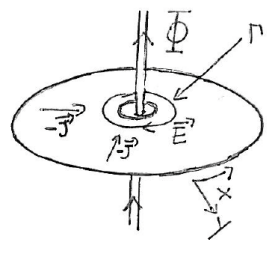
\includegraphics[width=0.3\linewidth]{Immagini - Capitolo 3/Gedanken experiment.png}
    \caption{dispositivo di Hall immerso in un campo magnetico.}
    \label{fig: Gedanken experiment}
\end{figure}

\subsection{Gauge simmetrico}
In questo caso, introducendo direttamente le variabili adimensionali
\begin{equation}
    l \equiv \sqrt{\frac{\hbar}{eB}},\quad y' \equiv \frac{y}{l},\quad x' \equiv \frac{x}{l},\quad p'_{x,y} = \frac{lp_{x,y}}{\hbar},
\end{equation}
l'hamiltoniana risulta essere
\begin{equation}
    \hatH' \equiv \frac{\hatH}{\hbar\omega_c} = \frac{1}{2}\bigg[\bigg(-i\frac{\p}{\p x'} - \frac{y'}{2}\bigg)^2 + \bigg(-i\frac{\p}{\p y'} + \frac{x'}{2}\bigg)^2\bigg].
\end{equation}
Definendo adesso le variabili complesse
\begin{equation}
    z = x' - iy' = re^{-i\theta},\quad \zbar  = x' + iy' = re^{i\theta},
\end{equation}
le derivate che compaiono nell'espressione di $\hatH'$ diventano
\begin{equation}
    \frac{\p}{\p x'} = \frac{\p}{\p z} + \frac{\p}{\p \zbar },\quad \frac{\p}{\p y'} = -i\bigg(\frac{\p}{\p z} - \frac{\p}{\p \zbar }\bigg).
\end{equation}
\begin{notz}
    La ragione per cui si usa questa convenzione per $z$ è che le funzioni d'onda dello stato fondamentale di Landau dipendono solo da $z$, a parte un fattore gaussiano $\exp{(-z\zbar /4)}$.
\end{notz}
Riscrivendo adesso l'hamiltoniana come
\begin{equation}
    \begin{split}
        \hatH' &= \frac{1}{2} + \frac{1}{2}\bigg[\bigg(-i\frac{\p}{\p y'} + \frac{x'}{2}\bigg) - i\bigg(-i\frac{\p}{\p x'} - \frac{y'}{2}\bigg)\bigg] \\
        &\times\bigg[\bigg(-i\frac{\p}{\p y'} + \frac{x'}{2}\bigg) + i\bigg(-i\frac{\p}{\p x'} - \frac{y'}{2}\bigg)\bigg],
    \end{split}
\end{equation}
si possono definire gli operatori 
\begin{align}
    \frac{1}{\sqrt{2}}\bigg[\bigg(-i\frac{\p}{\p y'} + \frac{x'}{2}\bigg) - i\bigg(-i\frac{\p}{\p x'} - \frac{y'}{2}\bigg)\bigg] &= \frac{1}{\sqrt{2}}\bigg(-2\frac{\p}{\p z} + \frac{\zbar }{2}\bigg) \equiv \hataT, \\
    \frac{1}{\sqrt{2}}\bigg[\bigg(-i\frac{\p}{\p y'} + \frac{x'}{2}\bigg) + i\bigg(-i\frac{\p}{\p x'} - \frac{y'}{2}\bigg)\bigg] &= \frac{1}{\sqrt{2}}\bigg(2\frac{\p}{\p \zbar} + \frac{z}{2}\bigg) \equiv \hata,
\end{align}
tali da soddisfare la relazione di commutazione 
\begin{equation}
    \comm{\hata}{\hataT} = 1,
\end{equation}
così da rendere l'hamiltoniana della forma
\begin{equation}
    \hatH' = \hataT\hata + \frac{1}{2}.
\end{equation}
Definendo lo stato di vuoto $\kO$ come $\hata\kO = 0$, si introduce la funzione d'onda $\eta_0(z,\zbar )$ cosicché 
\begin{equation}
\label{eq: funzione d'onda gauge simmetrico}
    \frac{1}{\sqrt{2}}\bigg(2\frac{\p}{\p \zbar } + \frac{z}{2}\bigg)\eta_0(z,\zbar ) = 0,
\end{equation}
che è equivalente a quanto detto nel formalismo di Schr\"odinger. Risolvendo poi l'equazione appena trovata
\begin{align}
    \frac{\p}{\p\zbar }\eta_0(z,\zbar) &= -\frac{z}{4}\eta_0(z,\zbar) \\
    \frac{\p}{\p\zbar}\log{\eta_0(z,\zbar)} &= -\frac{z}{4},
\end{align}
si ottiene
\begin{equation}
    \eta_0(z,\zbar) = \frac{1}{\sqrt{2\pi}}P(z)e^{-z\zbar/4},
\end{equation}
dove $P(z)$ è una funzione generica analitica in $z \in \C$, cioè una funzione non singolare intera che è possibile sviluppare sulla base $\{z^m\}$ con $m \ge 0$. A tale scopo, si osserva che gli operatori 
\begin{equation}
    \hatbT = \frac{1}{\sqrt{2}}\bigg(-2\frac{\p}{\p\zbar} + \frac{z}{2} \bigg),\quad \hatb = \frac{1}{\sqrt{2}}\bigg(2\frac{\p}{\p z} + \frac{\zbar}{2} \bigg) 
\end{equation}
commutano con gli operatori $\hata$, $\hataT$ e l'hamiltoniana $\hatH'$, per cui 
\begin{equation}
    \comm{\hatb}{\hatbT} = 1.
\end{equation}
Pertanto, si introduce lo stato annichilato simultaneamente dagli operatori $\hatb$ e $\hata$ tale per cui $\hatb\ket{0,0} = 0$, ossia che abbia la forma trovata in equazione \eqref{eq: funzione d'onda gauge simmetrico}, perciò
\begin{equation}
    \frac{1}{\sqrt{2}}\bigg(2\frac{\p}{\p z} + \frac{\zbar}{2} \bigg)\eta_{0,0}(z,\zbar) = \bigg[\frac{1}{\sqrt{2}}\bigg(\frac{\zbar}{2} - \frac{\zbar}{2}\bigg)P(z) + \sqrt{2}\frac{\p P(z)}{\p z}\bigg]\frac{e^{-z\zbar/4}}{\sqrt{2\pi}} = 0,
\end{equation}
da cui si trova che $P(z) = 1$. Analogamente, l'operatore $\hatbT$ agisce su questo stato come $\hatbT\ket{0,0} = \ket{0,1}$, per cui
\begin{equation}
    -\frac{1}{\sqrt{2}}\bigg(2\frac{\p}{\p\zbar} + \frac{z}{2} \bigg)\eta_{0,0}(z,\zbar) = \frac{z}{\sqrt{2}}\eta_{0,0}(z,\zbar) \equiv \eta_{0,1}(z,\zbar),
\end{equation}
o più in generale come
\begin{equation}
    \frac{(\hatbT)^m}{\sqrt{m!}}\ket{0,0} = \ket{0,m},
\end{equation}
per cui 
\begin{equation}
    \frac{(\hatbT)^m}{\sqrt{m!}}\eta_{0,0}(z,\zbar) = \frac{z^me^{-z\zbar/4}}{\sqrt{2\pi2^mm!}} = \eta_{0,m}(z,\zbar).
\end{equation}
Nel caso del gauge di Landau, si era trovato che per una geometria periodica le traiettorie riempiono lo spazio ma sono spaziate per il principio di esclusione di Pauli, similmente per una geometria a disco si possono graficare le traiettorie semi-classiche per ogni $n$ corrispondenti ai picchi della gaussiana, dove il raggio di ogni orbita è proporzionale ad $m^{1/2}$. La componente del momento angolare nella direzione $z$ è 
\begin{equation}
    \hatL' \equiv \frac{\hatL}{\hbar} = -i\frac{\p}{\p\theta},
\end{equation}
per cui
\begin{equation}
    z\frac{\p}{\p z} - \zbar\frac{\p}{\p \zbar} = \hatbT\hatb - \hataT\hata,
\end{equation}
dove il termine a primo membro corrisponde alla differenza tra il momento angolare trasportato dalla parte olomorfa, $\p/\p z$, e quello trasportato dalla parte anti-olomorfa, $\p/\p\zbar$, mentre nel termine a secondo membro $\hatbT\hatb$ aumenta $n$ ed $m$ mentre $\hataT\hata$ aumenta $n$ ma diminuisce $m$. Dato che gli operatori $\hatH$ e $\hatL$ commutano possono essere diagonalizzati simultaneamente. Gli stati costruiti sono autostati di $\hatL'$ con autovalore $-m$ con $m = [-n,\infty) \subset \Z$, ad esempio
\begin{equation}
    \hatL'\eta_{0,m}(z\zbar) = N\bigg(\zbar\frac{\p}{\p\zbar} - z\frac{\p}{\p z}\bigg)(z^me^{-z\zbar/4}) = -m\eta_{0,m}(z\zbar).
\end{equation}
Analogamente, gli autostati di $\hatH'$ per $n$ ed $m$ generici sono
\begin{equation}
    \ket{n,m} = \frac{(\hatbT)^{n+m}(\hataT)^n}{\sqrt{(n + m)!}\sqrt{n!}}\ket{0,0}
\end{equation}
con 
\begin{equation}
    \eta_{n,m}(z,\zbar) = N_{n,m}\bigg(\frac{z}{2} - 2\frac{\p}{\p\zbar}\bigg)^{n + m}\bigg(\frac{\zbar}{2} - 2\frac{\p}{\p z}\bigg)^ne^{-z\zbar/4}
\end{equation}
dove
\begin{equation}
    N_{n,m} = \frac{1}{\sqrt{2\pi 2^{m + 2n}n!(n + m)!}},
\end{equation}
che può essere riscritta in forma più compatta come
\begin{equation}
    \eta_{n,m}(z\zbar) = \frac{(-1)^n}{\sqrt{2\pi}}\sqrt{\frac{n!}{2^m(n + m)!}}e^{-r^2/4}z^mL_n^m\bigg(\frac{r^2}{4}\bigg),\quad r^2 \equiv z\zbar,
\end{equation}
dove $L^m_n$ sono i polinomi di Laguerre, la quale è effettivamente soluzione dell'oscillatore armonico in due dimensioni. 

Ignorando i fattori di normalizzazoine nel seguito, si consideri adesso la base di funzioni d'onda con momento angolare definito 
\begin{equation}
\label{eq: funzione d'onda singolo elettrico gauge simmetrico}
    \psi_m = z^me^{-|z|^2/4},\quad |\psi_m|^2 = |z|^{2m}e^{-|z|^2/2},
\end{equation}
il cui massimo di probabilità si può trovare ponendo
\begin{equation}
    \frac{\p|\psi_m|^2}{\p|z|} = (2m|z|^{2m - 1} - |z|^{2m + 1})e^{-|z|^2/2} = 0,
\end{equation}
da cui si trova che il raggio delle traiettorie è dato da 
\begin{equation}
    |z| = \sqrt{2m},
\end{equation}
per cui l'area delimitata da essa è 
\begin{equation}
    r^2\pi = 2ml^2\pi\quad\Longrightarrow\quad m = \frac{\pi r^2}{2\pi l^2},\quad |z| = \frac{r}{l}.
\end{equation}
Quindi, la traiettoria semi-classica dell'elettrone racchiude $m$ quanti di flusso $\Phi_0$; pertanto, all'elettrone dopo aver completato un'orbita viene associata una fase pari al numero di quanti di flusso $\Phi_0$ contenuti nell'area delimitata da tale orbita. Perciò la monodromia di $\psi_m$ è data dalla relazione
\begin{equation}
    \psi_m(z e^{2i\pi}) = \psi_m(z)e^{2i\pi m}.
\end{equation}
Nel gauge simmetrico le funzioni d'onda a singolo elettrone hanno la forma trovata in equazione \eqref{eq: funzione d'onda singolo elettrico gauge simmetrico}. Si tenta ora di costruire le funzioni d'onda per uno stato ad $N$ particelle. Per farlo si può usare il determinante di Slater così da avere una funzione d'onda totale, ad esempio per gli stati a due e tre particelle si hanno
\begin{equation}
    \begin{split}
        \psi^{(2)} &= 
        \begin{vmatrix}
            1 & 1 \\
            z_1 & z_2
        \end{vmatrix} 
        e^{-|z_1|^2/4}e^{-|z_2|^2/4} \\
        &= -(z_1 - z_2)\exp{\bigg[-\frac{1}{4}(|z_1|^2 + |z_2|^2)\bigg]},
    \end{split}
\end{equation}
\begin{equation}
    \begin{split}
        \psi^{(3)} &= 
        \begin{vmatrix}
            1 & 1 & 1 \\
            z_1 & z_2 & z_3 \\
            z_1^2 & z_2^2 & z_3^2
        \end{vmatrix} 
        e^{-|z_1|^2/4}e^{-|z_2|^2/4}e^{-|z_3|^2/4} \\
        &= [(z_2z_3^2 - z_3z_2^2) - (z_1z_3^2 - z_3z_1^2) + (z_1z_2^2 - z_2z_1^2)] \\
        &\times\exp{\bigg[-\frac{1}{4}(|z_1|^2 + |z_2|^2 + |z_3|^2)\bigg]} \\
        &= -\prod_{i<j}^3(z_i - z_j)\exp{\bigg[-\frac{1}{4}(|z_1|^2 + |z_2|^2 + |z_3|^2)\bigg]},
    \end{split}
\end{equation}
e così via. Quindi, in generale lo stato ad $N$ particelle è dato da
\begin{equation}
\label{eq: funzione d'onda stato ad N particelle gauge simmetrico}
    \psi \equiv \psi^{(N)} = \prod_{i<j}^N(z_i - z_j)\exp{\bigg(-\frac{1}{4}\nsum_j|z_j|^2\bigg)}
\end{equation}
e la probabilità non normalizzata per le particelle nel primo livello di Landau è
\begin{equation}
\label{eq: densità funzione d'onda stato ad N particelle gauge simmetrico}
    |\psi|^2 = \prod_{i<j}^N|z_i - z_j|^2\exp{\bigg(-\frac{1}{2}\nsum_j|z_j|^2\bigg)}.
\end{equation}
Quest'ultimo oggetto è molto complesso da trattare, è chiaro che il termine polinomiale diventi molto articolato se le particelle rimangono ben distanziate; d'altra parte il termine esponenziale tende a non farle disperdere troppo sfavorendo valori di $|z|$ troppo grandi. Per questo è difficile anche trovare una risposta a quesiti semplici come l'uniformità della densità delle particelle. Per risolvere il problema, Laughlin ha sviluppato un'analogia con la fisica del plasma che riesce a chiarire molte delle proprietà della funzione d'onda in equazione \eqref{eq: funzione d'onda stato ad N particelle gauge simmetrico}.

\subsubsection{Plasma interpretation}
Si introduce un funzione di partizione ipotetica 
\begin{equation}
    Z = \bigg(\int d^2z_1 \cdots \int d^2z_N\bigg)|\psi|^2,
\end{equation}
corrispondente alla funzione di partizione di un problema classico di meccanica statistica con peso di Boltzmann 
\begin{equation}
    |\psi|^2 = e^{-zU_C/\beta},
\end{equation}
dove
\begin{equation}
    U_C = \beta^2\sum_{i < j}^N(-\log{|z_i - z_j|}) + \frac{\beta}{4}\sum_{k=1}^N|z_k|^2 \equiv \beta^2U_{int}^{(N)} + \frac{\beta}{4}U_B^{(N)}.
\end{equation}
Il potenziale $U_C$ corrisponde all'energia potenziale di un plasma classico 2-dimensionale composto da particelle di carica $\beta$ in un background uniforme ``neutrilazzante''. Si può quindi utilizzare l'intuito per i sistemi classici di plasma per studiare la proprietà di $|\psi|^2$. Tramite le coordinate complesse $z$ e $\zbar$, il potenziale elettrostatico può essere riassunto nella forma
\begin{equation}
    \phi(z,\zbar) = -Q\log{\frac{|z|l}{r_0}}
\end{equation}
che, fissando $r_0 = l$ diventa
\begin{equation}
    \phi(z,\zbar) = -Q\log{|z|}.
\end{equation}
L'energia di interazione tra due cariche $Q$ poste a distanza $|z|$ è
\begin{equation}
    U^{(2)}_{int} = -Q^2\log{|z|},
\end{equation}
si vede quindi che il termine 
\begin{equation}
    U^{(N)}_{int} = \beta^2\sum_{i < j}^N(-\log{|z_i - z_j|})
\end{equation}
può essere interpretato come l'energia potenziale di interazione di un gas di $N$ particelle in due dimensioni con carica $\beta$. Bisogna però sempre tenere conto del fatto che non c'è nessun potenziale logaritmico nell'hamiltoniana di cui $\psi$ è soluzione. Per comprendere l'analogia con il plasma, si deve considerare che la carica $Q$ è data da
\begin{equation}
    \int d\vSigma \cdot \vE = 4\pi Q,
\end{equation}
poiché l'area della sfera è $4\pi r^2$, si ottengono
\begin{equation}
    \vE(\vr) = \frac{Q}{r^2}\hatr,\quad \phi(\vr) = \frac{Q}{r},
\end{equation}
tali per cui 
\begin{equation}
    \nabla \cdot \vE = -\nabla^2\phi.
\end{equation}
In due dimensioni 
\begin{equation}
    \int d\vSigma \cdot \vE = 2\pi Q,
\end{equation}
quindi si hanno 
\begin{equation}
    \vE(\vr) = \frac{Q}{r}\hatr,\quad \phi(\vr) = -Q\log{\frac{r}{r_0}}.
\end{equation}
Per comprendere il significato del termine $U_B^{(N)}$ si nota che 
\begin{equation}
    l\bigg(\frac{\p}{\p x} + i\frac{\p}{\p y}\bigg) = 2\frac{\p}{\p z},\quad l\bigg(\frac{\p}{\p x} - i\frac{\p}{\p y}\bigg) = 2\frac{\p}{\p \zbar},
\end{equation}
ossia
\begin{equation}
    \nabla^2 = \frac{\p^2}{\p x^2} + \frac{\p^2}{\p y^2} = \frac{4}{l^2}\frac{\p}{\p z}\frac{\p}{\p \zbar}.
\end{equation}
Quindi, si ha la relazione
\begin{equation}
    -\nabla^2 \frac{|z|^2}{4} = -\frac{1}{l^2}\frac{\p}{\p z}\frac{\p}{\p \zbar}(z\zbar) = -\frac{1}{l^2} = 2\pi\rho_B\quad\Longrightarrow\quad \rho_B = \frac{1}{2\pi l^2}.
\end{equation}
Tale equazione può essere interpretata come l'equazione di Poisson associata ad una distribuzione omogenea di carica $\rho_B$, dove
\begin{equation}
    \phi_B(z,\zbar) = \frac{|z|^2}{4}
\end{equation}
corrisponde al potenziale associato a questa distribuzione di carica. L'energia potenziale di una particella con carica $Q$ a distanza $|z|$ dal centro del sistema è
\begin{equation}
    U_B^{(1)} = \frac{Q|z|^2}{4}.
\end{equation}
Il termine $U^{(N)}_B$ in $U_C$ 
\begin{equation}
    U_B^{(N)} = \frac{\beta}{4}\nsum_k|z_k|^2
\end{equation}
rappresenta quindi l'energia potenziale elettrostatica legata alla presenza di un background con densità di carica $\rho_B$. Supponendo ora di aggiungere un quanto di flusso $\Phi_0$ adiabaticamente a $z = 0$, come nel gedanken experiment di Laughlin, si ha
\begin{equation}
    \psi_m(z) \to \psi_{m + 1}(z) = z^{m + 1}e^{|z|^2/4},
\end{equation}
ossia l'elettrone si è spostato sull'orbita successiva. Per il sistema a molti elettroni questo corrisponde a
\begin{equation}
    \psi^{(N)} = \prod_{i < j}^N(z_i - z_j)\exp{\bigg({-\frac{1}{4}\nsum_k|z_k|^2}\bigg)} \to \bigg(\nprod_kz_k\bigg)\psi^{(N)}.
\end{equation}

\section{Effetto Hall frazionario}
Con la scoperta dell'effetto Hall frazionario con fattore di riempimento $\nu = 1/3$, Laughlin intuì immediatamente che altri valori di $\beta$ erano possibili ed erano in grado di descrivere il fluido quantistico di Hall a $\nu = 1/\beta$ con $\beta \in \N$ dispari. La funzione d'onda corrispondente è
\begin{equation}
    \psi_\beta^{(N)} = \prod_{i < j}^N(z_i - z_j)^\beta\exp{\bigg(-\frac{1}{4}\nsum_k|z_k|^2\bigg)}
\end{equation}
ed è completamente antisimmetrica e sviluppabile sulla base $\{z^me^{-|z|^2/4}\}^{\otimes N}$ delle funzioni d'onda del primo livello di Landau; in particolare, il termine $\prod_{i < j}(z_i - z_j)^\beta$ contiene solo fattori olomorfi $\{(z_i)^k\}$ con $k \in [0,N] \subset \N$. Si supponga di voler determinare la funzione d'onda a due elettroni con momento angolare del centro di massa $M$ e momento angolare relativo $m$. Trascurando il mixing dei livelli di Landau per $n \ge 1$, la funziona d'onda deve essere sviluppabile sulla base 
\begin{equation}
    \{z_1^{m_1}e^{-|z_1|^2/4}\} \otimes \{z_2^{m_2}e^{-|z_2|^2/4}\},
\end{equation}
ossia la parte esponenziale deve essere olomorfa in $z_1$ e $z_2$, per cui 
\begin{equation}
    \psi^{(2)} = F(z_1,z_2)\exp{\bigg[-\frac{1}{4}(|z_1|^2 + |z_2|^2)\bigg]}.
\end{equation}
La funzione d'onda deve essere separabile in una parte corrispondente al moto del centro di massa e in una parte legata al moto relativo, quindi
\begin{equation}
    \psi^{(2)}_{m,M} = f(z_1 - z_2)g(z_1 + z_2)\exp{\bigg[-\frac{1}{4}(|z_1|^2 + |z_2|^2)\bigg]}.
\end{equation}
Considerando la simmetria per rotazione 
\begin{equation}
    \begin{cases}
        f[(z_1 - z_2)e^{2i\pi}] = e^{2i\pi m}f(z_1 - z_2) \\
        g[(z_1 + z_2)e^{2i\pi}] = e^{2i\pi M}g(z_1 + z_2)
    \end{cases},
\end{equation}
l'unica soluzione possibile indipendentemente dal tipo di potenziale di interazione è
\begin{equation}
    \psi^{(2)}_{m,M} = (z_1 - z_2)^m(z_1 + z_2)^M\exp{\bigg[-\frac{1}{4}(|z_1|^2 + |z_2|^2)\bigg]},
\end{equation}
dove $m \in \N$ dispari. Considerando anche l'interazione a due corpi, l'energia corrispondente a tale stato è 
\begin{equation}
    E = \frac{\mybrakett{m,M}{\hatH_1 + \hatH_2 + \hatV_{12}}{m,M}}{\mybraket{m,M}{m,M}} = \hbar\omega_c + \frac{\mybrakett{m,M}{\hatV_{12}}{m,M}}{\mybraket{m,M}{m,M}},
\end{equation}
nel caso di interazione coulombiana
\begin{equation}
    E_{12}(m,M) = E_{12}(m) = e^2k\frac{\mybrakett{m,M}{|z|^{-1}}{m,M}}{\mybraket{m,M}{m,M}} = \frac{\sqrt{2}(2m)!}{2^{2m + 1}(m!)^2}e^2k,
\end{equation}
dove $k$ è la costante di Coulomb; in particolare, per $m \gg 1$ e usando l'approssimazione di Stirling il risultato è $E_{12}(m) \simeq 1/\sqrt{2m}$ dove $\sqrt{2m}$ è il raggio dell'orbita contenente $m$ quanti di flusso $\Phi_0$. Questo dimostra che i livelli energetici sono quantizzati come se fossero\ stati legati. In assenza di campo magnetico, la forza coulombiana repulsiva tende a far allontanare gli elettroni che perdono energia potenziale acquistando energia cinetica. In presenza di campo magnetico invece l'energia cinetica è quantizzata ed è pari a $\hbar\omega_c/2$ per ogni elettrone nel primo livello di Landau. Pertanto, gli elettroni non possono allontanarsi e formano stati legati con energia di legame $E_{12}$ positiva. In queste condizioni, a fissato fattore di riempimento $1/\beta$, il sistema presenta un gap di energia. Si consideri ad esempio $\nu = 1/3$, tutte le coppie di elettroni possiedono momento angolare relativo $m = 3$, per cui
\begin{equation}
    \psi^{(N)} = \prod_{i < j}^N(z_i - z_j)^3\exp{\bigg(-\frac{1}{4}\nsum_k|z_k|^2\bigg)}
\end{equation}
e uno stato eccitato corrisponderebbe quindi ad una transizione; ad esempio, $m = 3 \to m = 5$ per una coppia di elettroni $(12)$. Tuttavia, a fissato fattore di riempimento, un'altra coppia di elettroni deve transire $m'=3 \to m'=1$. Inoltre, poiché
\begin{align}
    \Delta E &= \Delta E_{12}(3 \to 5) + \Delta E_{12}(3 \to 1) \\
    &= E_{12}(5) - E_{12}(3) + E_{12}(1) - E_{12}(3) \\
    &= \frac{31\sqrt{2\pi}}{512}e^2k,
\end{align}
si ha una gap di energia $E_{12} > 0$ positivo e lo stato con $\nu = 1/3$ corrisponde quindi ad un fluido incomprimibile. La presenza di tale gap, come nel caso con $\nu = 1$, è cruciale per avere $\rho_{xx} = \sigma_{xx} = \rho_{yy} = \sigma_{yy} = 0$. 